% !TEX root = macfp_2017_gasphase.tex

\subsection{Case 4: Turbulent Wall Fires} \label{sec:wall_fires}

\subsubsection{Experiment}

Turbulent fire on a vertical surface is a canonical configuration representing the upward flame spread problem, typical in many practical fire scenarios. The FM Global vertical wall flame experiment selected for the first MaCFP workshop~\cite{Case4_EXP_1,Case4_EXP_2} is a series of meter-scale wall fires (the total heat release rate is several 100s of kW) realized by an array of vertically-stacked water-cooled porous gas burners with prescribed fuel supply rates. The setup conveniently decouples the gas-phase fire dynamics and corresponding heat transfer from the solid-phase pyrolysis, and thereby achieves a statistically steady-state condition ideal for experimental measurements and CFD model validation. The original goal of the experiment was to provide data to establish theoretical models and correlations for radiative and convective gas-to-solid heat transfer in wall fires. The fuel type and the fuel injection rate were varied in the tests. The total flame-to-wall heat flux as well as inward and outward flame radiation intensities were measured at different elevations. Other measurements included wall-normal profiles of gas temperature and flow velocity and vertical profiles of the soot depth. This experimental configuration provides MaCFP with the following: a canonical configuration that brings data on flame-wall interactions with realistic scales and buoyant turbulent flow conditions; a simplified statistically-stationary configuration that brings data on the different forms of heat transfer; and decoupled solid- and gas-phase processes through controlled fuel injection.

\subsubsection{Simulations}

Two groups submitted computational results for Case 4: FM Global~\cite{Case4_SIM_FMG} and NIST~\cite{Case4_SIM_NIST}. FM Global used FireFOAM version 2.2.x~\cite{FireFOAM}; NIST used an official release of FDS (version 6.5.3)~\cite{FDS}.

As discussed in section~\ref{sec:CGD}, the main challenge found in the design of a computational grid for LES simulations of the FM Global vertical wall flame experiment is to provide suitable grid resolution to capture the thin turbulent boundary layer flame. This requires millimeter-scale resolution. FM Global and NIST responded to this challenge in a similar way and adopted a 3-mm resolution in the near-wall flame region. In a previous study of the same wall fire configuration~\cite{Ren:2016}, this level of spatial resolution was found to be adequate for grid-resolved LES simulations ($i.e.$ for simulations that capture the wall gradients and are performed without using wall models). NIST chose to apply the 3-mm resolution in all directions and across the entire computational domain. FM Global chose a lower-cost computational grid and applied the 3-mm resolution in the wall-normal direction while using a 7.5-mm resolution in the spanwise and vertical directions (parallel to the wall) and also used a coarser mesh in the far field.

Additional differences in the numerical treatment of the wall flame experiment include differences in the choice of physical models (see section~\ref{sec:PM} for details on baseline choices). FM Global used the baseline configuration of FireFOAM except for using the WALE model~\cite{Ducros:1999} for subgrid-scale turbulence and for correct behavior in the near-wall region; the values of the global radiative loss fraction were prescribed using the measured values (to account for the radiation absorption from the fuel and cold soot in the near wall region, the prescribed values were chosen as 75\% of the values of the radiative loss fraction measured in corresponding wall-free configurations); in the solution of the RTE, the discretization of angular space used 16 angles. NIST used the baseline configuration of FDS except for using an emission/absorption treatment of the RTE based on a simplified soot formation model (using a prescribed soot yield) and a grey model for soot radiation as well as a wide-band (6 bands) model for gas radiation (with coefficients calibrated by the narrow-band model called RadCal~\cite{RadCal}); in the solution of the RTE, the discretization of angular space used 104 angles. Note that in its baseline configuration, FDS uses a Smagorinsky model with Van Driest wall functions~\cite{FDS_Math_Guide} to estimate a turbulent viscosity at the wall and a Nusselt-number-based convective heat transfer model to estimate the convective heat flux at the wall~\cite{FDS_Math_Guide}.

Interestingly, FM Global and NIST differ significantly in their near-wall treatment: while FM Global follows the modeling choices of Ref.~\cite{Ren:2016} and adopts a wall-resolved approach in which the wall convective heat flux is calculated by direct differentiation of the resolved temperature field (no wall model is used), NIST adopts a wall-modeled approach in which the wall convective heat flux is reconstructed by wall functions and Nusselt-number correlations. It is not clear whether the wall-modeled approach adopted by NIST converges towards a wall-resolved approach in case of sufficient grid resolution.

\begin{figure}
\centering
(a)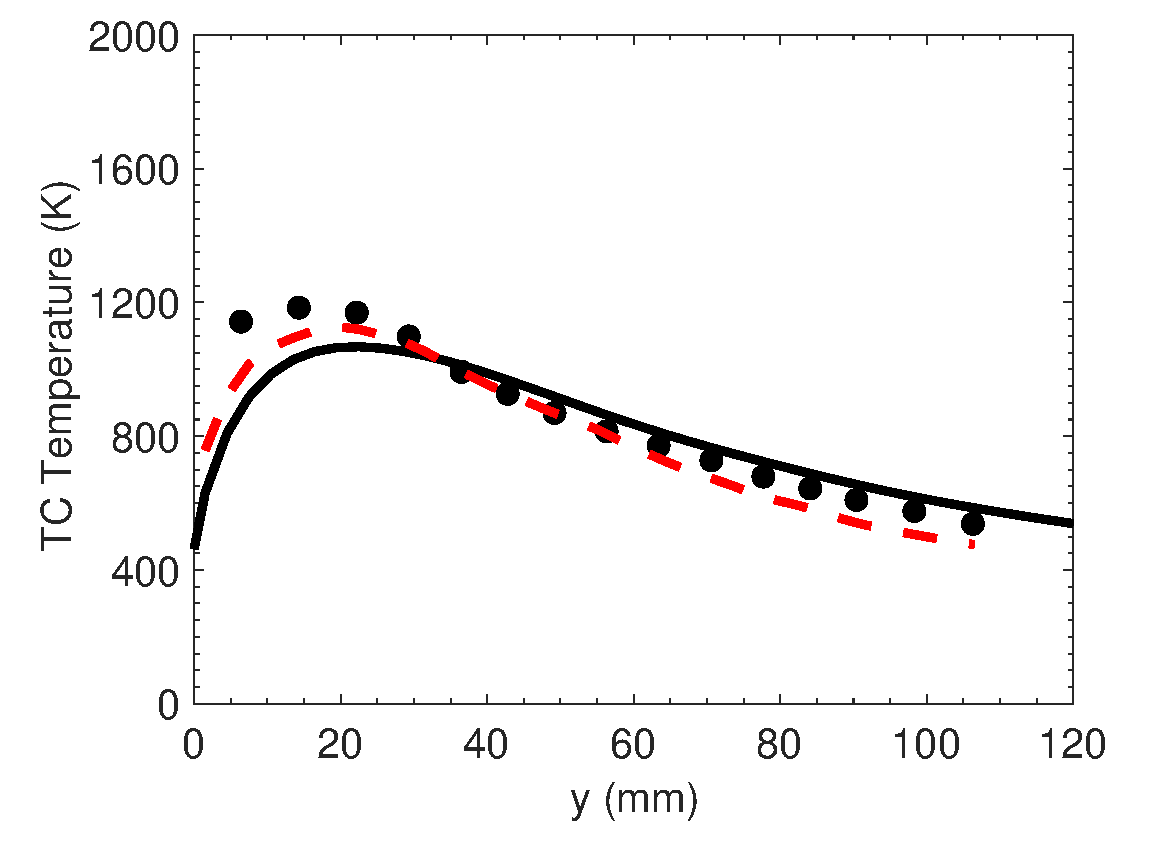
\includegraphics[height=2.2in]{Figures/Case4-Fig1a.pdf}
(b)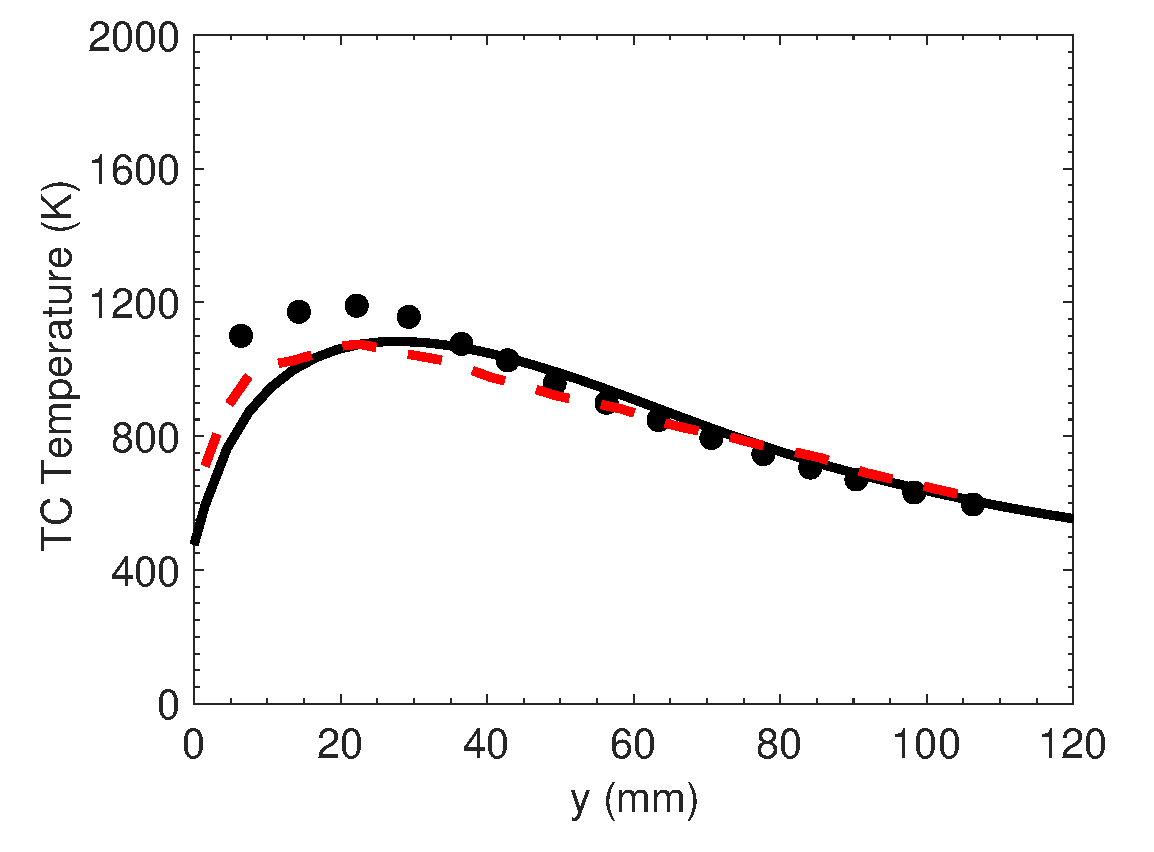
\includegraphics[height=2.2in]{Figures/Case4-Fig1b.pdf}
\caption{Case 4. Wall-normal variations of mean thermocouple temperature at $z$ = 0.77~cm and for a fuel supply rate equal to: (a) 12.68 g/m$^2/$s; (b) 17.05 g/m$^2/$s. Comparison between experimental data (black circles) and numerical results from FM Global (black solid line) and NIST (red dashed line). Case of a propylene flame.}
\label{fig:Case4-Fig1}
\end{figure}

\subsubsection{Summary}

We limit our discussion to the case of propylene fuel (additional results can be found in~\cite{MaCFP_wks_presentations}). Both FM Global and NIST simulations qualitatively reproduce the variations of the wall heat flux with vertical elevation as well as the variations of the wall heat flux in response to changes in the fuel supply rate. Figure~\ref{fig:Case4-Fig1} presents a representative sample of comparisons between measured and simulated thermocouple temperatures (note that in these comparisons, both FM Global and NIST simulations use a thermocouple model that is integrated inside the solvers and that uses the LES solution to simulate the deviations of thermocouple temperatures from gas temperatures). Figure~\ref{fig:Case4-Fig2} presents a sample of comparisons between measured and simulated wall heat fluxes. The NIST simulations overpredict the total heat flux by approximately 50\% in most scenarios. In contrast, the FM Global simulations shows good agreement with experimental data, a result that may be attributed to the choice of using a semi-empirical radiation model with an experimentally-determined global radiative loss fraction. These results suggest that even with a fine computational grid, a radiation treatment based on a simplified soot formation model combined with a grey model for soot radiation and a wide-band model for gas radiation is not sufficiently accurate to predict wall heat fluxes in a wall flame configuration. Note that because the experimental database does not include information on the convective and radiative components of the wall heat flux, this information was not extracted from the simulations. Future simulations of this case should analyze these components (see for instance Ref.~\cite{Ren:2016}) and also bring information on the relative weight of soot radiation and gas radiation.

\begin{figure}
\centering
(a)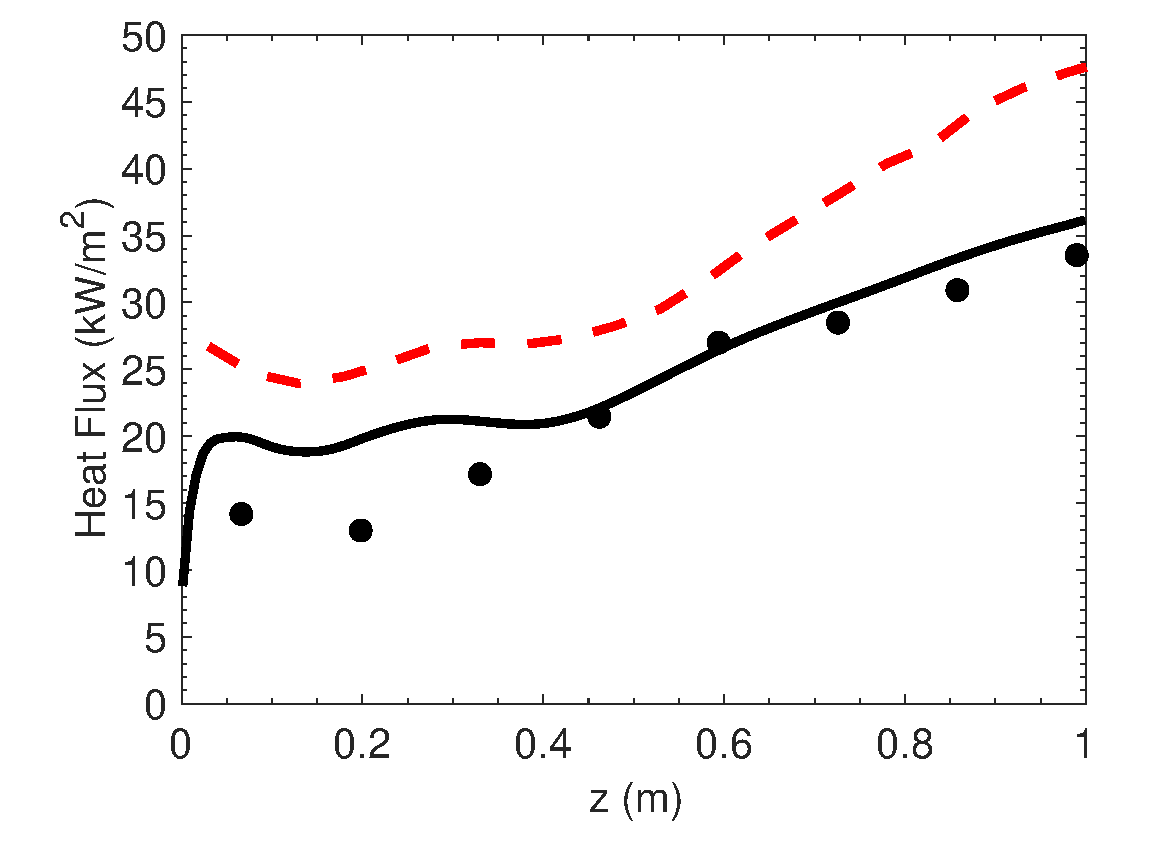
\includegraphics[height=2.2in]{Figures/Case4-Fig2a.pdf}
(b)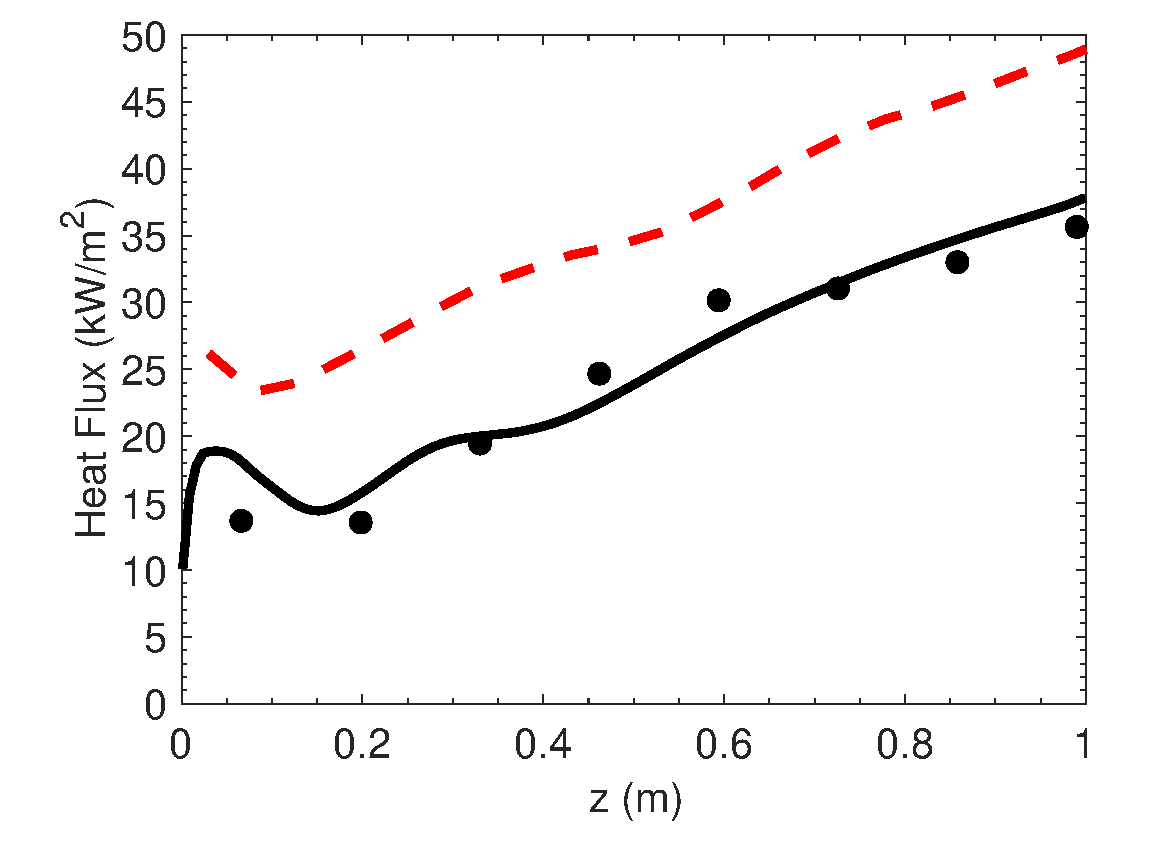
\includegraphics[height=2.2in]{Figures/Case4-Fig2b.pdf}
\caption{Case 4. Vertical variations of the mean total wall heat flux for a fuel supply rate equal to: (a) 12.68 g/m$^2/$s; (b) 17.05 g/m$^2/$s. See caption of Fig.~\ref{fig:Case4-Fig1}.}
\label{fig:Case4-Fig2}
\end{figure}

In closing, the experimental database describing the FM Global vertical wall flame experiment is quite unique because it brings fundamental information on gas-to-solid heat transfer processes that are a controlling factor in flame spread problems. There are also some limitations in the database that are worth pointing out for future studies: (1) the database is limited to temporal means and does not contain information on fluctuation magnitudes; (2) the thermal feedback is characterized in terms of a total wall heat flux but does not contain information on the convective and radiative components of the wall heat flux, nor on the soot and gas contributions to the radiative component of the wall heat flux.

Furthermore, as already pointed out in section~\ref{sec:gaseous_pool_fires}, it is worth noting that while research-level simulations may accept the computational cost associated with millimeter-scale resolution, engineering-level simulations will not accept that cost and will use coarser grids that require wall models. The development and evaluation of these models is part of the future objectives of MaCFP.


